\documentclass[a4paper,ngerman,oneside,titlepage,bibliography=totoc,11pt]{scrreprt}


\pagestyle{headings}

\usepackage{geometry}
\geometry{left=31mm, top=34mm, right=31mm, bottom=34mm}

\renewcommand{\ttdefault}{lmtt}
\linespread{1.06} %font

\usepackage[font=small,labelfont=bf]{caption} %caption, caption-font
\usepackage{subcaption}
\usepackage{amsmath, amsthm, amssymb, amsbsy}
\usepackage{mathtools}
\usepackage{color}
\usepackage{booktabs}
\usepackage{microtype}
\usepackage{natbib}
\usepackage[ngerman]{babel}
\usepackage[utf8]{inputenc} % für Umlaute (ansinew Editor, utf8 bei Texniccenter/Texmaker)
\usepackage[T1]{fontenc} % korrekte Trennung von Umlauten

\usepackage[hyphens]{url}
\usepackage{hyperref}
\usepackage{animate}
\usepackage{rotating}
\usepackage{longtable}
\usepackage{setspace}
\onehalfspacing



\begin{document}



\begin{titlepage}

\newcommand{\HRule}{\rule{\linewidth}{0.5mm}} % Defines a new command for the horizontal lines, change thickness here

\center % Center everything on the page
 
%----------------------------------------------------------------------------------------
%	HEADING SECTIONS
%----------------------------------------------------------------------------------------

\LARGE Ludwig-Maximilians-Universität München\\[0.2cm] % Name of your university/college
\LARGE Institut für Statistik\\[5mm]% Major heading such as course name
\large Projekt im Rahmen des statistischen Consultings\\[6mm]
% Minor heading such as course title

%----------------------------------------------------------------------------------------
%	TITLE SECTION
%----------------------------------------------------------------------------------------

\HRule \\[0.4cm]
{ \huge \bfseries Internationaler Waffenhandel:\vspace{-1.5mm} Die Anwendung neuer Verfahren der\\[1mm] statistischen Netzwerkanalyse}\\[5mm]
{ Eine Netzwerkanalyse des internationalen Kleinwaffenhandels 1992 - 2011}\\
{ Kooperation mit dem Lehrstuhl für empirische Politikforschung}\\[0.4cm] % Title of your document
\HRule \\[1.5cm]
 
%----------------------------------------------------------------------------------------
%	AUTHOR SECTION
%----------------------------------------------------------------------------------------

\begin{minipage}[t]{0.4\textwidth}
\begin{flushleft} \large
\emph{Autor:}\\[2mm]
Felix Loewe\\
loewe.felix@gmail.com\\[5mm]


\end{flushleft}
\end{minipage}
~
\begin{minipage}[t]{0.4\textwidth}
\begin{flushright} \large
\emph{Projektpartner:}\\[2mm]
Prof. Dr. Paul W. Thurner\\[6mm]

\emph{Betreuer:}\\[2mm]
Prof. Dr. Göran Kauermann\\[6mm]
\end{flushright}
\end{minipage}\\[4.5cm]

\end{titlepage}




\begin{abstract}


\begin{center}
{\it \bf Abstract} 
\end{center}

hier kommt noch das abstract rein
 


\end{abstract}




\tableofcontents




\chapter{Einführung}

Was ist das Besondere an der statistischen Analyse von Netzwerken? Erstens stellen sie durch ihre Abhängigkeitsstruktur relationale Daten dar. Gewöhnliche Datensätze mit $i = 1, ..., N$ Beobachtungen werden zumeist mit der Annahme analysiert, dass die $n$ Beobachtungen unabhängig voneinander beobachtet werden. Bei Netzwerkdaten ist das nicht der Fall. Hier stehen die Beobachtungen, oft genannt \emph{Akteure} des Netzwerkes, in Beziehung zueinander. Besteht eine Beziehung zwischen den Beobachtungen, können diese nicht mehr als unabhängig angesehen werden. In ähnlicher Sichtweise wird auch eine nicht-bestehende Beziehungen nicht ignoriert, sondern so angesehen, dass individuenspezifische oder netzwerkspezifische Effekte diese verursacht haben können.

Das Bestehen oder Nicht-Bestehen einer Beziehung ist die Netzwerkstruktur (\emph{Abhängigkeitsstruktur}), die zusätzlich zu den Daten eines gewöhnlichen Datensatzes besteht. Die Abhängigkeitsstruktur wird durch die Adjazenzmatrix $Y_{ij} \in N \times N$ ausgedrückt.

Bei der Analyse des Waffenhandels wird aus der Beziehung ein Handel und aus den Akteuren die liefernden und belieferten Länder.

Die Arbeit ist wie folgt aufgebaut. Im ersten Kapitel erfolgt eine kurze Wiederholung der Begriffe aus der Graphentheorie. Netzwerkspezifische Begriffe sowie deskriptive Maßzahlen werden theoretisch eingeführt. Darauf folgt eine Erläuterung der Datengrundlage der NISAT Datenbank mit den daraus resultierenden Möglichkeiten und Einschränkungen. Im dritten Abschnitt wird der Datensatz deskriptiv analysiert. Im vierten Abschnitt erfolgt die Modellierung per ERGMs.





\section{Zusammenfassung der Graphentheorie}

Um Netzwerkdaten statistisch analysieren zu können, muss die Abhängigkeitsstruktur der Daten adäquat modelliert werden. Eine grundlegende mathematische Theorie, die verwendet wird, um \emph{relationale Daten} zu beschreiben, ist die Graphentheorie. Im Rahmen dieses Kapitels wird nur auf die wichtigsten Aspekte der Graphentheorie eingegangen. Es handelt sich im Wesentlichen um eine Zusammenfassung der Kaptitels 2.1 und 4.2 aus \citet{kol09}.

\subsection{Graph - Grundlegende Begriffe}

Ein \emph{Graph} $G = (V,E)$ ist die mathematische Beschreibung eines Netzwerkes. 

Er besteht aus einer Knotenmenge $V$ und einer Kantenmenge $E$. Ein \emph{Knoten} $v$ repräsentiert einen Akteur des Netzwerkes. Eine \emph{Kante} $e$ verbindet zwei Akteure und kennzeichnet eine Beziehung zwischen ihnen.
Die Anzahl der Knoten $N_V = |V|$ wird üblicherweise als kleiner unendlich vorausgesetzt. Häufig benennt man die Knoten eines Netzwerkes einfach nach ihrem ihren Index $i = 1, ..., N_V$
Eine Kante $\{i,j\}$ ist ein Element der Menge $E$ und  beschreibt die Verbindung zwischen Knoten $i$ und $j$. 
Man unterschiedet zwischen \emph{gerichteten} und \emph{ungerichteten} Graphen. Ein ungerichteter Graph setzt eine symmetrische Beziehung zwischen den Akteuren voraus. Akteur $i$ steht also zu Akteur $j$ in der gleichen Beziehung wie $j$ zu $i$ (z.B. Arbeitskollege). Bei einem gerichteten Graphen hingegen ist die Richtung der Beziehung entscheidend. Dies ist in unserem Datensatz der Fall. Wir unterschieden zwischen Exporteur und Importeur eines Handels. Die Kante $\{i,j\}$ ist hier also von der Kante $\{j,i\}$ zu unterscheiden. Einen gerichteten Graphen nennt man auch \emph{Digraph}.

Per Definition enthält ein Graph weder Schleifen noch multiple Kanten. Von einer \emph{Schleife} spricht man, wenn eine Kante $\{i,j\}$ den gleichen Anfangs- und Endpunkt besitzt ($i = j$). Von einer \emph{multiplen Kante} spricht man, falls zwischen zwei Knoten mehrere Verbindungen bestehen. Enthält ein Netzwerk solche Eigenschaften spricht man von einem \emph{Multigraphen} ansonsten von einem \emph{einfachen Graphen}.

Betrachtet man die Anzahl der möglichen Kanten eines Graphen, die später als Benchmark dafür auftaucht, wie dicht ein Graph sein kann, so wird ersichtlich, dass diese Anzahl für einen einfachen ungerichteten Graphen kleiner ist als die Anzahl der möglichen Kanten eines gerichteten Graphen. Für einen einfachen ungerichteten Graphen ist sie gegeben durch $V_H(V_H-1)/2$. Ein gerichteter Graph kann logischerweise maximal die doppelte Anzahl an Kanten enthalten.

Notwendigerweise gibt es einige Begriffe um über die Konnektivität von Graphen zu reden. Am gebräuchlichsten ist das Prinzip der \emph{Nachbarschaft}. Zwei Knoten $ i,j \in V$ gelten als benachbart wenn sie von einer Kante $\{i,j\} \in E$ verbunden werden. Zwei Kanten wiederum gelten als benachbart, wenn sie durch einen gemeinsamen Knoten aus $V$ verbunden werden.

Ein sogenannter \emph{Weg} auf einem Graphen von $v_0$ nach $v_l$ bezeichnet die alternierende Sequenz $\{v_0, e_1, v_1, e_2, ..., v_{l-1}, e_l, v_l\}$. $l$ bezeichnet hierbei die Länge des Weges. Weiter beschreibt ein \emph{Pfad} einen Weg ohne wiederholte Knoten oder Kanten. Als \emph{Distanz} zwischen zwei Knoten eines Graphen definiert man die Länge des kürzesten Pfades der sie verbindet. Die Länge der längsten Distanz innerhalb eines Graphen nennt man \emph{Durchmesser} eines Graphen.

\subsection{Degree-Verteilung}
Ein weiterer Begriff ist der des \emph{Degree} eines Knotens $d_v$, definiert als die Anzahl der Kanten, die den Knoten $v$ enthalten. Die \emph{Degree-Sequenz} eines Graphen $G$ ist die Sequenz die entsteht, wenn man alle Knoten-Degrees in aufsteigender Reihenfolge sortiert. Nun definiert man $f_d$ als den Anteil der Knoten $v \in V$ mit Degree $d_v = d$. Die Reihe $\{f_d\}_{d \geq 0}$ heißt \emph{Degree-Verteilung} von $G$. 

Bei einem gerichteten Graphen unterscheidet man zwischen \emph{In-Degree} ($d_v^{in}$) und \emph{Out-Degree} ($d_v^{out}$) und zählt die Kanten die zu einem Knoten hin, beziehungsweise von ihm weg laufen. Die oben genannten Begriffe lassen sich hierfür trivial erweitern.

\subsection{Nachbarschaftsmatrix}

Die Struktur eines Graphen ist vollständig bestimmt durch seine binäre und symmetrische\emph{ Nachbarschaftsmatrix} (auch \emph{Adjazenzmatrix}) $A \in |V| \times |V|$, wobei $a_{ij} = 1$ falls zwischen Knoten $i$ und Knoten $j$ eine Kante besteht und $a_{ij} = 0$ sonst. Diese Matrix hat einige nützliche Eigenschaften. Zum Beispiel ergibt die Zeilensumme $A_{i,} = \sum_j{A_{ij}}$ den Degree $d_i$ von Knoten $i$.  
Bei gerichteten Graphen besteht ein Unterschied zwischen der Kante $(i,j)$ und der Kante $(j,i)$. Die Adjazenzmatrix ist hier nicht symmetrisch. Allerdings enthält sie immer noch ähnliche Informationen wie zum Beispiel $A_{i,} = d_i^{out}$ und $A_{,j} = d_j^{in}$

\subsection{Zentralität}
Viele Fragestellungen der Netzwerkanalyse drehen sich darum welche Akteure auf eine bestimmte Weise besonders wichtig für ihr Netzwerk sind. Maßzahlen der Zentralität sind dafür gedacht um diese Wichtigkeit der Knoten zu quantifizieren und dadurch die Beantwortungen solcher Fragestellungen zu vereinfachen. Das wichtigste Konzept in diesem Zusammenhang, den Degree haben wir bereits kennen gelernt. Zusätzlich führe ich nun kurz die Begriffen Closeness und Betweeness Zentralität ein.

Bei der \emph{Closeness} Zentralität wird ein Knoten als zentral angesehen, falls er vielen anderen Knoten "`nahe"' ist.
Man verwendet für dieses Maß die inverse der Summe der Distanz eines Knotens zu allen anderen,
$$ c_{Cl}(v)=\frac{1}{\sum_{u \in V}{dist(v,u)}}, $$
wobei $dist(v,u)$ die Distanz zwischen den Knoten $v$ und $u$ bezeichnet. Um eine Vergleichbarkeit mit anderen Graphen und Zentralitätsmaßen herzustellen normalisiert man die Maßzahl in das Intervall $[0,1]$ indem man mit dem Faktor $N_v - 1$ multipliziert.

Ein anderes Konzept basiert auf dem Gedanken, dass die Wichtigkeit eines Knotens darauf beruht, wie oft sich ein Knoten auf der Verbindung zwischen anderen Paaren von Knoten befindet. Knoten die auf vielen Pfaden eines Netzwerkes sitzen, werden als wichtig für die Kommunikation innerhalb des Netzwerkes angesehen. 
Die \emph{Betweeness} Zentralität wird deswegen üblicherweise definiert als
$$ c_{B}(v)= \sum_{s \neq t \neq v \in V} {\frac{\sigma(s,t|v)}{\sigma(s,t)}}, $$
wobei $\sigma(s,t|v)$ die Anzahl der kürzesten Pfade zwischen $s$ und $t$ ist, die durch $v$ verlaufen und $\sigma(s,t) = \sum_v{\sigma(s,t|v)}$.

\subsection{Dichte}
Die \emph{Dichte} eines Netzwerkes ist die Anzahl der Kanten des Netzwerkes, geteilt durch die mögliche Anzahl an Kanten des Netzwerkes. Es ergibt sich der Term $$den(G) = \frac{|E_G|}{|V_G|(|V_G|-1)/2}$$ für die Dichte. Die Dichte liegt zwischen null und eins. Es sei angemerkt, dass die Dichte auch als Skalierung des durchschnittlichen Degrees $\bar{d}(G)$ angesehen werden kann, denn $den(G) = (|V_G| - 1) \bar{d}(G)$.

\section{Datengrundlage}
Die Datengrundlage für das Kleinwaffenhandelsnetzwerk ist die \emph{NISAT} (Norwegian Initiative on Small Arms Transfers) Datenbank. Das Peace Research Institute Oslo (PRIO) ist der Auftraggeber dieser Datenbank. Die Datenbank enthält Daten über den legalen und illegalen Handel von Kleinwaffen. Der abgedeckte Zeitraum beträgt die Jahre 1992 bis 2011. Berichtet wird hierin von insgesamt 239 Ländern und 109522 Waffentransaktionen.

Es folgt eine genauere Beschreibung der Datenbank. Die Daten liegen in der Form einer gerichteten Kanten-Liste vor. Das bedeutet jede Zeile im Datensatz entspricht einem Handel zwischen einem exportierenden und einem importierenden Land. Zusätzliche Attribute sind die Correlates of War Codes der jeweiligen Länder, der monetäre Wert des Handels in US Dollar, der gehandelte Waffentyp , die berichtende Datenquelle sowie das Jahr in dem der Handel stattgefunden hat.
Bei der Analyse dieser Daten erkennt man schnell folgende Probleme:

Da nach Waffentypen unterschieden wird, existieren in den einzelnen Jahren multiple Kanten. Das bedeutet zwischen zwei Ländern werden im gleichen Jahr mehrere Handel in der gleichen Richtung aufgeführt. Diese wurden für die weitere Analyse zusammengefasst indem der Wert der Lieferungen schlicht addiert wurde.

Der Datensatz enthält Schleifen. Das heißt manche Länder liefern Waffen an sich selbst. Da es hierfür keine sinnvolle inhaltliche Erklärung gibt wurden die entsprechenden Beobachtungen gelöscht. Eine Liste der gelöschten Kanten befindet sich im Anhang.

\chapter{Deskriptive Analyse}

\section{Degree Sequenz}

\label{sec:degree}
\begin{figure}[ht]
	\centering
		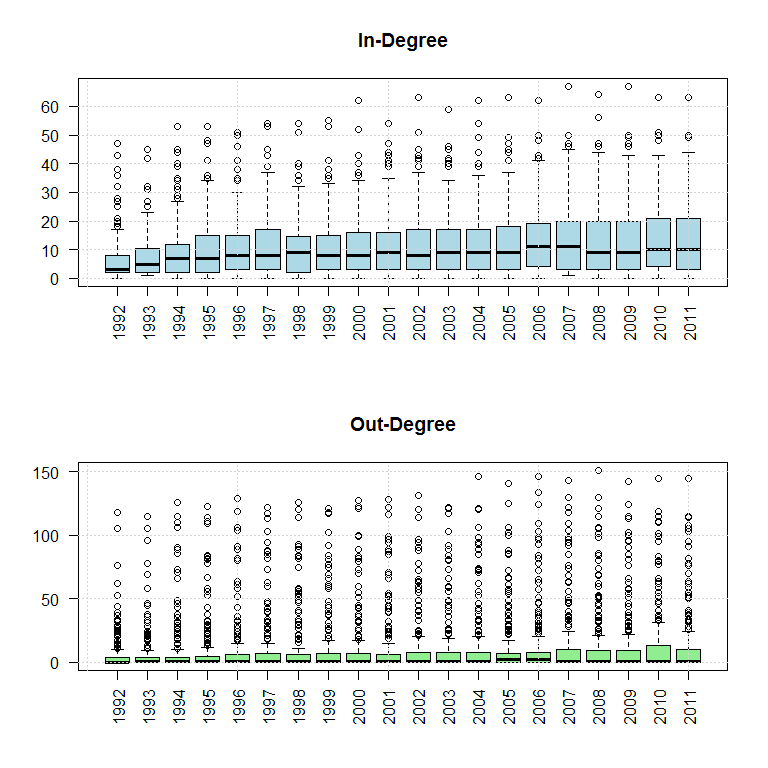
\includegraphics[width=1.00\textwidth]{Grafiken/ts_degree.png}
	\caption{Boxplot für In- und Out-Degree in den Jahren 1992-2011}
	\label{fig:ts_degree}
\end{figure}

Eine erste nützliche Analyse um die Struktur des Netzwerkes zu erfassen, ist die Betrachtung der Knoten-Degrees. Im Falle eines gerichteten Netzwerkes unterschiedet man zwischen In-Degree und Out-Degree. Inhaltlich interpretiert entspricht dies den Anzahlen der Importe und Exporte eines Landes pro Jahr. Hierzu betrachten wir Abbildung \ref{fig:ts_degree}. Sie zeigt zu jedem im Datensatz enthaltenen Jahr je einen Boxplot der In-Degrees und Out-Degrees aller Länder. Innerhalb der farblich gekennzeichneten Box liegen jeweils die mittleren 50 Prozent der entsprechenden Daten. Der mittlere schwarze Strich in jeder Box kennzeichnet den Median, und damit den Wert, unter dem genau die Hälfte aller Werte liegt.

Betrachtet man zuerst die Boxplots zum In-Degree, so stellt man fest, dass die breite der Box über die Jahre zunimmt. Im Jahr 1992 reicht sie lediglich von zwei bis acht, während sie sich im Jahr 2011 von drei bis 21 erstreckt. Auch der Median steigt über diesen Zeitraum von drei auf zehn. Daraus lässt sich schließen, dass die mittlere Anzahl Importpartner eines einzelnen Landes über die Zeit größer geworden ist. Auffallend sind in allen Jahren einige mit Kreisen markierte Ausreißer,
die aus bis zu 67 verschiedenen Ländern im gleichen Jahr Waffen beziehen.

Bei den Boxplots zum Out-Degree fallen sofort die eher kleinen Boxen auf. Übereinstimmend in allen Jahren exportieren mindestens 25 Prozent der Länder überhaupt keine Waffen, und 50 Prozent der Länder an höchstens 2 andere Staaten. Allerdings gibt auch in allen Jahren eine recht große Anzahl von Ausreißern mit hohem Out-Degree mit bis zu 150 belieferten Staaten. 

Die Betrachtung der Degrees legt nahe, dass der Kleinwaffenhandel von einigen wenigen Akteuren dominiert wird, während die große Masse der restlichen Staaten eher einen geringen Einfluss auf die Geschehnisse hat. Diesen wichtigen Akteuren wenden wir uns in Abschnitt \ref{sec:top-akteure} zu.


\begin{figure}[htbp]
	\centering
		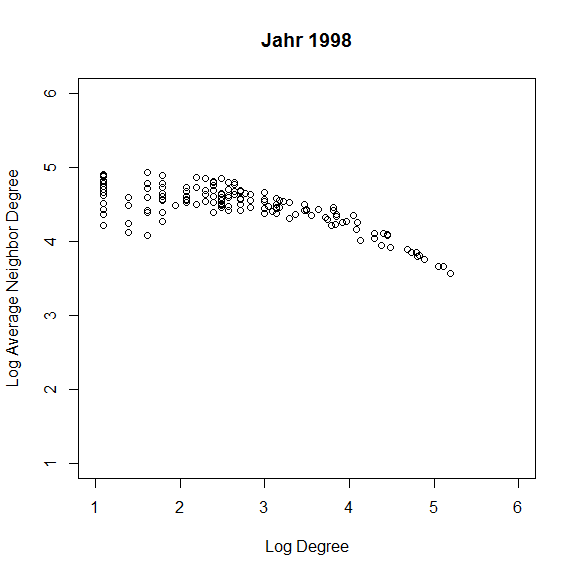
\includegraphics[width=0.60\textwidth]{Grafiken/and.png}
	\caption{Average nearest Neighbor Degree am Beispiel von 1998}
	\label{fig:and}
\end{figure}

Interessante Einblicke in die Zusammenhänge innerhalb eines Netzwerkes lassen sich auch generieren, indem man den Degree eines Knoten mit dem seiner Nachbarn vergleicht. Zwei Netzwerke mit gleicher Degree-Sequenz können dennoch unterschiedliche Strukturen besitzen, falls sich die Knoten der Netzwerke darin unterscheiden mit welchen anderen Knoten sie sich bevorzugt verbinden. Hierzu betrachten wir Abbildung \ref{fig:and}. Hier ist das Jahr 1998 exemplarisch ausgewählt. Dem logarithmierten Knoten Degree auf der X-Achse ist der logarithmierte durchschnittliche Degree der Nachbar auf der Y-Achse gegenübergestellt. Man erkennt, dass sich Knoten mit geringerem Degree tendenziell eher mit Knoten mit hohen Degree verbinden als Knoten, die selbst einen hohen Degree besitzen. Zentrale Akteure des Netzwerkes handeln also eher mit kleineren Akteuren des Netzwerkes als mit anderen zentralen Akteuren.


\section{Handelswerte}


Betrachtet man die Gewichte der Kanten, in diesem Fall die monetären Handelswerte, so fällt einem ein deutliches Ungleichgewicht auf. Wie Abbildung \ref{fig:ts_value} zeigt ist die Summe der 1\% teuersten Waffenhandel über alle Jahre hinweg ähnlich der Summe der 99\% billigsten. Einige wenige große Waffentransaktionen wiegen also alle restlichen in ihrem monetären Gewicht auf. 
\begin{figure}[ht]
	\centering
		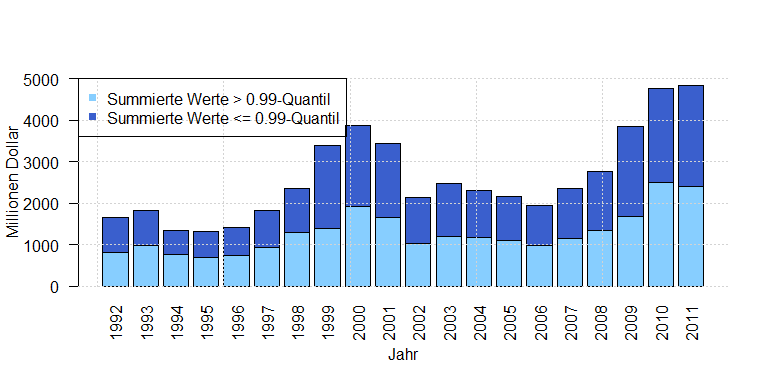
\includegraphics[width=0.7\textwidth]{Grafiken/ts_value.png}
	\caption{Vergleich der 1\% teuersten Waffenkäufe mit den 99\% billigsten in den Jahren 1992-2011}
	\label{fig:ts_value}
\end{figure}

\section{Top-Akteure}
\label{sec:top-akteure}
In Abschnitt \ref{sec:degree} wurde anhand der Degree-Verteilungen gezeigt, dass der Kleinwaffenhandel von einigen wenigen Nationen dominiert wird, die sich deutlich von der großen Masse der restlichen Akteure abheben. Diese sollen in diesem Abschnitt ermittelt werden. Hierzu werden in Tabelle \ref{tab:tops} diejenigen Nationen aufgelistet, die über den Zeitraum von 20 Jahren das größte Import- und Exportvolumen, gemessen am Geldwert der gehandelten Waffen, aufweisen. 

\begin{table}[ht]

\centering

\begin{minipage}[t]{0.48\textwidth}
\footnotesize
\begin{tabular}{rlr}
  \hline
 Platz & Land & Exportvol. [Mrd.]\\ 
  \hline
1 & USA & 9.2\\ 
  2 & Italy & 7.9 \\ 
  3 & Germany & 4.6 \\ 
  4 & Brazil & 3.7 \\ 
  5 & Austria & 2.7 \\ 
  6 & United Kingdom & 2 \\ 
  7 & Belgium & 1.8 \\ 
  8 & Switzerland & 1.5 \\ 
  9 & Russia & 1.4 \\ 
  10 & Czech Republic & 1.4 \\ 
   \hline
	\end{tabular}
	\end{minipage}	
\hfill	
\begin{minipage}[t]{0.48\textwidth}	
\footnotesize
\begin{tabular}{rlr}
  \hline
 Platz & Land & Importvol. [Mrd.]\\ 
  \hline
1 & USA & 16\\ 
  2 & Germany & 2.3\\ 
  3 & France & 2.3\\ 
  4 & Canada & 1.9 \\ 
  5 & United Kingdom & 1.8\\  
  6 & Saudi Arabia & 1.7\\ 
  7 & Belgium & 1.2\\ 
  8 & Spain & 1.2\\ 
  9 & Australia & 1.2\\ 
  10 & Turkey & 1\\ 
   \hline
\end{tabular}
\end{minipage}
\caption{Summierte Handelswerte der Top-Importeure und Top-Exporteure des Netzwerkes von 1992 bis 2011}
\label{tab:tops}
\end{table}


Es ist ersichtlich, dass die Vereinigten Staaten von Amerika mit 9.2 Milliarden Dollar am meisten Waffen exportiert. Italien steht mit 7.9 Milliarden Dollar Exportvolumen an zweiter Stelle. Deutschland exportiert mit 4.6 Milliarden Dollar gehandelten Waffen am drittmeisten. Auf dem vierten und fünften Platz folgen die Länder Brasilien und Österreich. Ab dem sechsten Platz erfolgen nur noch unwesentliche Verringerungen des Exportvolumens im Bereich von 2 bis 1 Milliarde Dollar. Hierin befinden sich Nationen wie Großbritannien, Belgien, die Schweiz, Russland und die tschechische Republik. 

		
Auch bei den Importen steht die USA an erster Stelle. Die Nation gibt mit 16 Milliarden Dollar mehr für den Import von Kleinwaffen aus als die 9 nachfolgenden Länder zusammen. Deutschland und Frankreich teilen sich mit 2.3 Milliarden Dollar Importvolumen den zweiten Platz. Auf der vierten Stelle befindet sich Kanada mit einem Importvolumen von circa 2 Milliarden Dollar. Großbritannien verwendet 1.8 Milliarden Dollar, um Waffen zu exportieren, und Saudi Arabien 1.7 Milliarden Dollar. Auf dem siebten, achten, neunten und zehnten Platz sehen wir ähnliche Exportausgaben von circa 1.2 bis 1 Milliarde Dollar. Dies sind die Länder Belgien, Spanien, Australien und Türkei.

Anschließend interessiert, ob sich die Zusammensetzung der Top-Exporteure/ Importeure über die Jahre verändert. Hierfür betrachten wir Abbildung \ref{fig:ts_tops}. 
In der ersten Grafik sind die Handelsvolumen in Millionen US Dollar der fünf Top-Exporteure über den Zeitraum 1992-2011 dargestellt. Die USA ist in fast allen Jahren der Waffenexporteur mit den höchsten monetären Volumen. Sie wird nur in wenigen Jahren von Italien übertroffen. Deutschland, Brasilien und Österreich exportieren in allen Jahren deutlich weniger Waffenwert als die USA. Auffällig ist ein relativ konstanter Verlauf der Zeitreihen im Zeitraum von 1992 bis ca 2001, während danach bei allen Ländern ein kräftiger Anstieg der Handelswerte feststellbar ist. Deutschland, Brasilien und vor allem Italien zeigen allerdings ab circa 2008 wiederum einen abfallenden Trend.
Die zweite und die dritte Grafik aus Abbildung \ref{fig:ts_tops} zeigt die Handelsvolumen der Top-Importeure. Die USA ist hier unangefochten an der Spitze. Sie importiert Kleinwaffen im Wert zwischen circa 400 und 1600 Millionen US Dollar pro Jahr während die restlichen Akteure höchstens Kleinwaffen im Wert von circa 250 Millionen Dollar pro Jahr importieren. Ähnlich wie bei den Exportzeitreihen ist auch hier ein relativ konstanter Verlauf bis circa 2001 zu beobachten während die Ausgaben in den nachfolgenden Jahren kontinuierlich ansteigen. Die USA verringerte ihre Importausgaben ab dem Jahr 2007 jedoch wieder deutlich. 

\begin{figure}[ht]
	\centering
		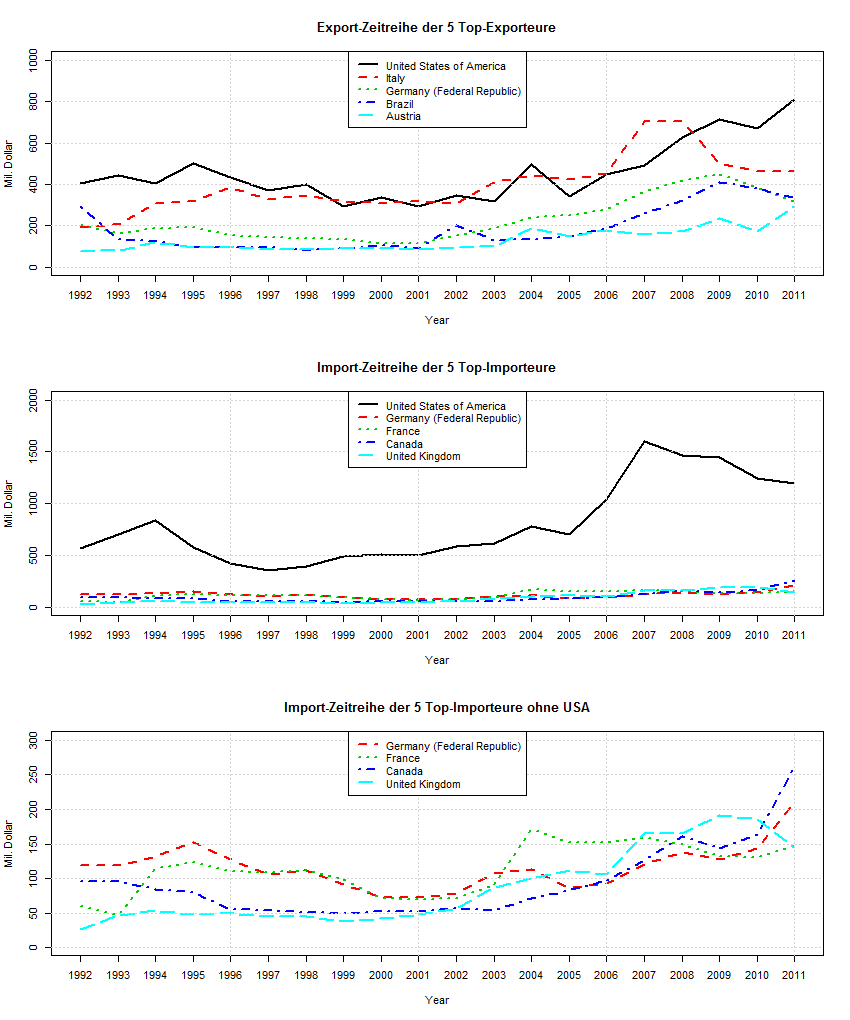
\includegraphics[width= 0.8\textwidth]{Grafiken/ts_tops.png}
	\caption{Zeitreihen der jährlichen Handelswerte der Top-Exporteure/Importeure von 1992 bis 2011}
	\label{fig:ts_tops}
\end{figure}
Eine andere Methode, um zentrale Akteure des Netzwerkes zu identifizieren ist sich die Degree-Sequenz der Netzwerkknoten zu betrachten. Welche Knoten (Länder) besitzen sowohl einen hohen In-Degree als auch einen hohen Out-Degree und können somit als zentrale Akteure des Handelsnetzwerkes identifiziert werden?
\begin{figure}[ht]
	\centering
		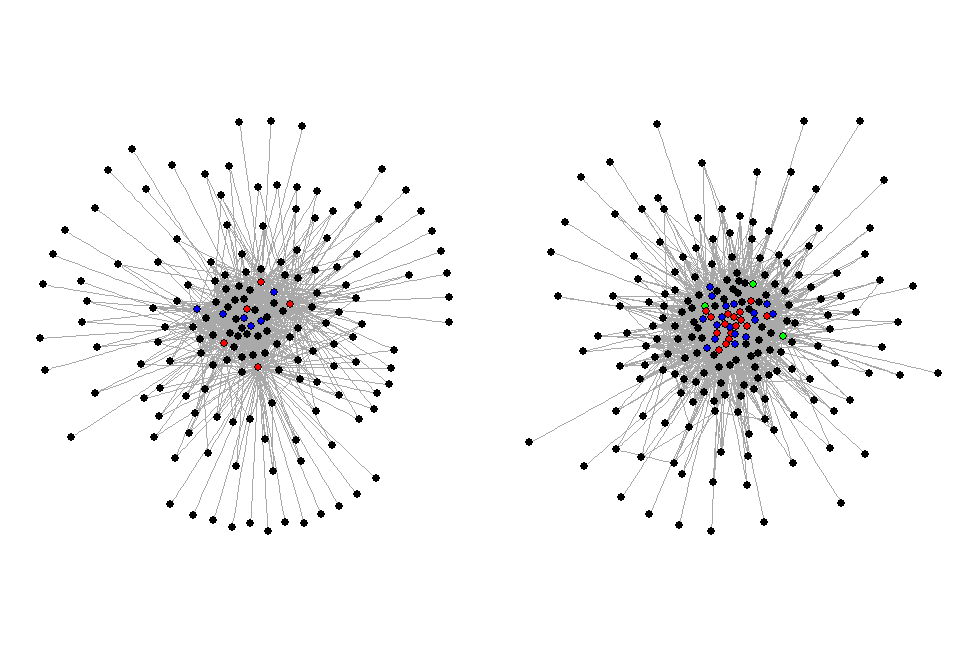
\includegraphics[width=0.90\textwidth]{Grafiken/ts_network.png}
	\caption{Visualisierung des Netzwerkes 1992 (l.) und 2011(r)}
	\label{fig:ts_network}
\end{figure}

Abbildung \ref{fig:ts_network} zeigt hierzu das Gesamte Netzwerk in den Jahren 1992 und 2011. Jeder Punkt stellt ein am Waffenhandel beteiligtes Land dar. Ein Pfeil zwischen den beiden Ländern symbolisiert einen Handel. Länder die aus mindestens 30 anderen Ländern Waffen beziehen sind grün, Länder die in mindestens 30 andere Länder Waffen liefern sind blau, und Akteure die beide Bedingungen erfüllen sind rot eingefärbt. Die beiden Tabellen in Tabelle \ref{tab:ZentrAkt} listen diese für das Jahr 1992 und das Jahr 2011 auf. Man erkennt, dass die Anzahl der "`großen Akteure"' auf dem Kleinwaffenmarkt über die Zeit deutlich zugenommen hat.


\begin{table}[ht]
\centering
\footnotesize
\begin{minipage}[t]{0.48\textwidth}

\begin{center}
1992
\end{center}

\begin{tabular}{rlr}
  \hline
 Land 											& In-Degree & Out-Degree\\ 
  \hline
 Switzerland 								& 32				& 76\\ 
 USA 	& 43				& 105\\ 
 Germany & 47				& 118\\ 
 Spain 											& 36				& 62\\ 
 Sweden 										& 38 				& 33\\ 
   \hline

\end{tabular}
\end{minipage}
\hfill	
\begin{minipage}[t]{0.48\textwidth}

\begin{center}
2011
\end{center}

\begin{tabular}{rlr}
  \hline
 Land 						& In-Degree & Out-Degree\\ 
  \hline
 Switzerland 			& 41				& 103\\ 
 USA					 		& 63				& 145\\ 
 Finland 					& 34				& 70\\ 
 Italy 						& 39 				& 114\\ 
 France						& 41				& 82\\ 
 Poland						& 32				& 34\\
 Czech Rep.		& 37				& 105\\
 Germany					& 50				& 115\\
 UK		& 44				& 95\\
 Norway						& 32				& 39\\
 Spain  					& 37				& 91\\
 Canada						& 49				& 78\\
 Austria					& 41				& 108\\
 South Africa			& 34				& 32\\
 Belgium					& 31				& 64\\
 Australia				& 39				& 51\\
   \hline

\end{tabular}
\end{minipage}
\caption{Zentrale Akteure des Netzwerkes  1992 und 2011} 
\label{tab:ZentrAkt}
	\end{table}



\section{Netzwerkmaßzahlen}
\begin{figure}[ht]
	\centering
		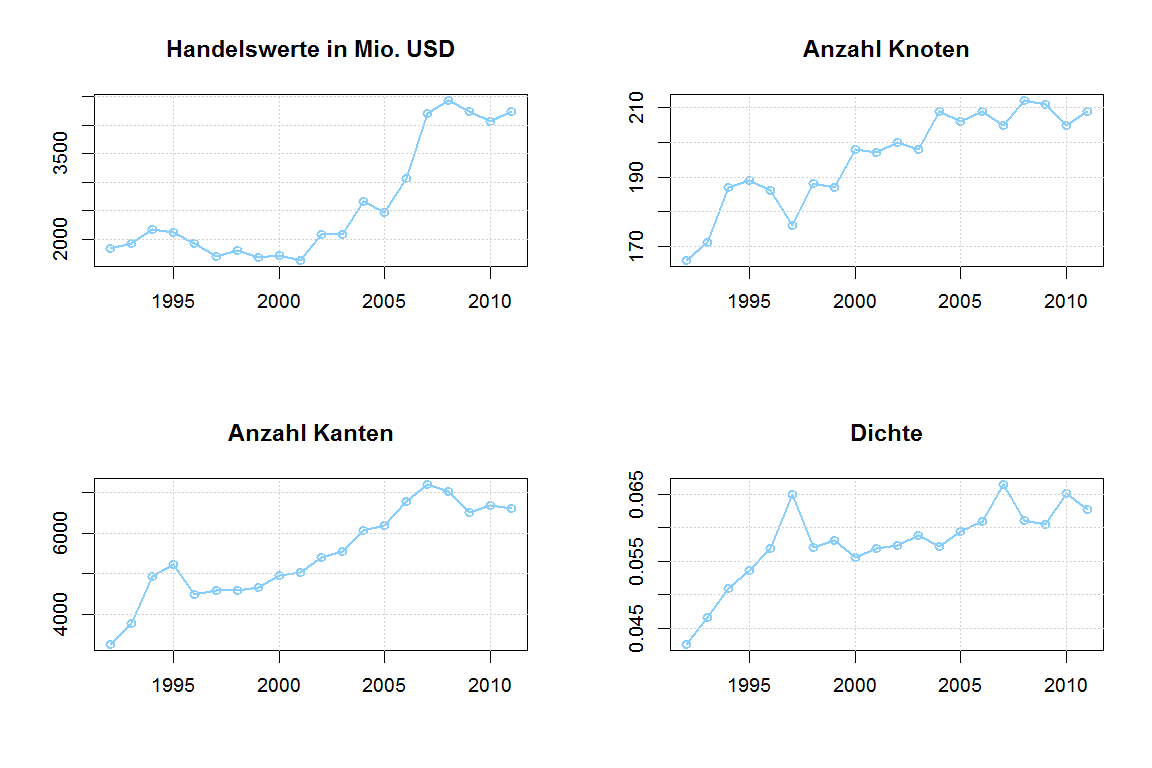
\includegraphics[width=0.9\textwidth]{Grafiken/ts_descriptives.png}
	\caption{Deskriptive Maßzahlen des Kleinwaffenhandelsnetzwerkes 1992-2011}
	\label{fig:ts_descriptives}
\end{figure}
Als zweites erfolgt eine Darstellung grundlegender deskriptiver Netzwerkmaßzahlen, um das Kleinwaffenhandelsnetzwerk zu beschreiben. Die Maßzahlen werden für jedes Jahr berechnet und als Zeitreihe dargestellt, um die zeitliche Entwicklung des Netzwerkes zu visualisieren. 
Abbildung \ref{fig:ts_descriptives} zeigt die zeitliche Entwicklung  von Handelswert, Knotenanzahl, Kantenanzahl und Dichte des Netzwerkes. Betrachtet man zuerst die Zeitreihe der Handelswerte so stellt man fest, dass diese in den Jahren 1992 bis 2001 relativ konstant zwischen 1.5 und 2.5 Milliarden US Dollar verweilt, nach 2001 jedoch bis auf ca 4.5 Milliarden im Jahr 2008 ansteigt und anschließend auf diesem Level konstant bleibt.
Die Zeitreihe der Anzahl der am Waffenhandel beteiligten Nationen steigt recht gleichmäßig zwischen Jahren 1992 und 2011. Lediglich zwischen 1993 und 1994 ist ein außergewöhnlich starker Anstieg von 170 auf 187 zu beobachten. Im Jahr 1997 ist die Anzahl der am Waffenhandel beteiligten Nationen auffallend von 186 auf 176 gesunken. Allerdings stellt sich gleich im Folgejahr wieder die ursprüngliche Anzahl ein. Das Maximum der Zeitreihe liegt mit 212 Nationen im Jahr 2008.
Auch die Anzahl der Netzwerkkanten die der Anzahl der vollzogenen Waffentransaktionen zeigt einen regelmäßig steigenden Trend von ca 3000 im Jahr 1992 bis ca 7000 im Jahr 2011. Auch hier erkennen wir einen sprunghaften Anstieg zwischen 1993 und 1994 sowie ein einknicken im Jahr 1996.
Die Dichte des Netzwerkes steigt in den Jahren 1992-1997 rasch von ca 0.04 auf 0.065 und stagniert anschließend auf einem Level zwischen 0.065 und 0.055.

%Die Dichte eines Netzwerkes ist die Anzahl der Kanten des Netzwerkes, geteilt durch die mögliche Anzahl an Kanten des Netzwerkes. Das Kleinwaffenhandelsnetzwerk $G_{NISAT}$ ist ein gerichteter Multigraph mit Schleifen. Da für Multigraphen keine Dichte definiert ist, wird der Graph mit dem Befehl \ttt{simplify(G_Nisat)} auf einen einfachen Graphen reduziert. Die Schleifen im Datensatz werden in der Berechnung der Dichte entfernt. Es ergibt sich der Term $den(G_{NISAT}) = \frac{E_V}{N_H(N_H-1)/2}$ für die Dichte.

\newpage
\section{Visualisierungen}



In diesem Abschnitt wird versucht durch verschiedene Visualisierungen des Netzwerkes einen Überblick über mögliche Strukturen und Zusammenhänge des Kleinwaffenhandels zu erhalten. Da das Netzwerk recht groß ist erscheint es ratsam, die Länder in Gruppen aufzuteilen. Hierdurch erreicht man eine bessere Übersichtlichkeit der Grafiken. Dies geschieht mit Hilfe des R-Pakets \emph{countrycode} \citep{countrycode}. Mit Hilfe der im Datensatz gegeben Correlates of War Country Codes und Zuordnungen der Vereinten Nationen weist dieses Paket jedem Land einen Kontinent und eine Region zu. In den beiden Grafiken \ref{fig:cont} und \ref{fig:reg} ist die Größe der Knoten proportional zum jeweiligen Degree (In-Degree + Out-Degree) gewählt. Die Breite der Kanten wiederum ist proportional zum monetären Wert der Handelsströme zwischen zwei Kontinenten beziehungsweise Regionen gewählt. Die Positionierung der Knoten wurde zur besseren Vergleichbarkeit der Jahre untereinander fixiert.

\begin{figure}[ht]
\centering
\animategraphics[scale=0.7, controls]{1}{Grafiken/Cont_Ani/cont}{1}{20}
\caption{Handelsströme zwischen den Kontinenten von 1992-2011}
\label{fig:cont}
\end{figure}

In Abbildung \ref{fig:cont} erkennt man, dass Europa durchgängig mit dem größten Kreis markiert ist, also an mehr Handelsaktionen als die anderen Kontinente beteiligt ist. Amerika und Asien folgen auf den nächsten beiden Plätzen. Die Dicke der Kanten und damit der Geldfluss zwischen den Kontinenten variiert stark zwischen den Jahren. Hier ist kein gleichbleibendes Muster zu erkennen.

\begin{figure}[ht]
\centering
\animategraphics[scale=0.7, controls]{1}{Grafiken/Reg_Ani/reg}{1}{20}
\caption{Handelsströme zwischen den Regionen von 1992-2011}
\label{fig:reg}
\end{figure}

In Abbildung \ref{fig:reg} zeigt sich ein ähnliches Bild. Die europäischen Regionen und Nordamerika scheinen die aktivsten Handelspartner zu sein, während immer wieder auch zwischen eher weniger aktiven Regionen große Geldsummen fließen und hier auch wieder kein konstantes Muster zu erkennen ist.  

\chapter{Exponential Random Graph Model}
Abschnitt \ref{sec:defmod} folgt \citep{hunter2008ergm}.
Abschnitt \ref{sec:simzuf} folgt \citep[Kapitel 12.2]{lkr12}.
Abschnitt \ref{sec:modpar} folgt \citep[Kapitel 12.3]{lkr12}.

\section{Definition des Modells}
\label{sec:defmod}
Sie $X$ eine Zufallsmatrix und repräsentiere die Nachbarschaftsmatrix eines Netzwerkes und $\mathcal{X}$ die Menge aller möglichen binären Netzwerke. Typischerweise fixiert man die Anzahl der Knoten auf einen festen Wert $n$. Dann ist $\mathcal{X}$ die Menge aller $n \times n$ Matritzen deren Einträge entweder eins oder null sind und die auf ihrer Diagonalen nur Nuller besitzen. Da das $ij$-te Element von $X$ eine Kante zwischen Knoten $i$ und $j$ entspricht, garantiert die letzte Eigenschaft, dass das Netzwerk frei von Schleifen ist. Bei einem ungerichteten Netzwerk ist $X$ eine symmetrische Matrix.
Die Verteilung von $X$ lässt sich in folgender Form ausdrücken:
\begin{equation}
P_{\theta, \mathcal{X}}(X = x) = \frac{exp\left\{\theta^T g(x)\right\}}{\kappa(\theta, \mathcal{X})}
\label{eq:ergm}
\end{equation}
mit

\begin{itemize}
	\item $x \in X$
	\item $\theta \in \Omega \subset \mathbb{R}^q$ ... Vektor der Modellparameter
	\item $g(x)$ ... q-Vektor aus Statistiken basierend auf der Nachbarschaftsmatrix $X$
\end{itemize}
Ersetzt man $g(x)$ aus Gleichung \ref{eq:ergm} durch $g(x,Y)$ so ermöglicht man die Aufnahme von zusätzlichen exogenen Informationen $Y$ über das Netzwerk (siehe Kapitel \ref{sec:exkov}). $\kappa(\theta, \mathcal{X}) = \sum_{z in \mathcal{X}}{exp\left\{\theta^T g(x)\right\}}$ ist ein Normalisierungsfaktor, der sicherstellt, dass es sich bei Gleichung \ref{eq:ergm} um eine Wahrscheinlichkeitsverteilung handelt. Die genaue Spezifikation von $\mathcal{X}$ ist problematisch, da $\mathcal{X}$ alle möglichen Netzwerke enthalten muss. Da aber bei $n$ Knoten bereits $2^{n(n-1)}$ verschiedene Netzwerke denkbar sind erhält mal schnell unvorstellbar große Anzahlen von möglichen Netzwerken die den Umgang mit  $\kappa(\theta, \mathcal{X})$ zum entscheidenden Problem dieses Modells werden lassen. Da eine analytische Lösung des Modells hierdurch oft unmöglich ist, benötigt man Methoden um durch simulationgestütze Verfahren geeignete Schätzer entwickeln zu können. Hiermit beschäftigen sich die nächsten beiden Kapitel.

\subsection{Simulation von Zufallsgraphen}
\label{sec:simzuf}
Die Simulation von Zufallsgraphen aus einer Zielverteilung $P_\theta(x)$ basiert auf dem Makrov Chain Monte Carlo (MCMC) Algorithmus. Hierbei erstellt man eine Sequenz von M Graphen. Der letzte dieser Graphen entspringt dann der Zielverteilung, dem ERGM. Hierbei beginnt man mit einem beliebigen Netzwerk mit fester Knotenzahl $N$. Nun sucht man sich ein zufälliges Knotenpaar und fügt eine Verbindung hinzu, beziehungsweise entfernt eine bestehende Verbindung. Besitzt der so erhaltene Graph nun eine höhere Wahrscheinlichkeit als der vorherige wird er akzeptiert. Besitzt der Graph eine geringere Wahrscheinlichkeit, so wird er mit einer Wahrscheinlichkeit akzeptiert, die proportional zum Verhältnis aus den Wahrscheinlichkeiten von altem und neuem Graph ist. Wird dieser Vorgang häufig genug iteriert, so erhält man ein zufälliges Netzwerk, das aus der Zielverteilung gezogen wurde. Alle vorherigen Ziehungen nennt man \emph{Burn In}. Der Burn In wird benötigt, damit der Algorithmus den beliebig gewählten Anfangszustand "`vergessen"' kann. Bei ausreichend großem Burn In ist das gezogene Netzwerk unabhängig von Startpunkt und jedes nach ihm gezogene Netzwerk entspringt ebenfalls der Zielverteilung.
Genauer gesagt benutzen wir einen Metropolis Algorithmus. Wir erstellen eine Sequenz von Graphen $X^{(0)}, X^{(1)}, ..., X^{(M-1)}, X^{(M)}$. Im $m$-ten Iterationsschritt wird hierbei folgendermaßen vorgegangen:

\begin{enumerate}
	\item Aus dem aktuellen Graphen $x^{(m-1)}$ wird ein zufälliges Knotenpaar $i,j$ ($i,j \in 1, ...,N$) ausgewählt.
	\item Der vorgeschlagene Graph $x^* = x^{(m-1)}$ bis auf $x_{ij}^{(m-1)} = 1 - x_{ij}^{(m-1)}$.
	\item Der vorgeschlagene Graph wird mit der Wahrscheinlichkeit $min\{1, \frac{P_{\theta}(x^*)}{P_{\theta}(x^{m-1})}\}$ akzeptiert.
	\item Bei Akzeptanz entspricht der neue Graph $x^m = x^*$ und sonst $x^m = x^{m-1}$.
\end{enumerate}

Hierbei ist für das Verhältnis von $\frac{P_{\theta}(x^*)}{P_{\theta}(x^{m-1})}$ die Berechnung der Change-Statistiken ausreichend, denn

\begin{align*}
log\{\frac{P_{\theta}(x^*)}{P_{\theta}(x^{m-1})}\} &= log\{P(X_{ij} = 1-x_{ij}^{m-1}|X_{-ij}=x_{ij}^{m-1}\} \\
																										&= \theta_1(z_1(x^*) - z_1(x^{m-1})) + \theta_2(z_2(x^*) - z_2(x^{m-1}))\\   																									& + ... + \theta_p(z_p(x^*) - z_p(x^{m-1}))
\end{align*}.

Diese Methode kann computional optimiert werden, indem man zum Beispiel größere Update-Schritte oder Update-Schritte mit ungleichen Gewichten zulässt.

Will man mehrere Graphen aus der selben Verteilung ziehen, so kann die gleiche Kette verwendet werden. Dafür lässt man zwischen den Beobachteten Graphen jeweils $k$ Iterationen aus. Den Wert von $k$ nennt man \emph{thinning}. Die gezogenen Graphen sind dann allerdings eine abhängige Stichprobe und man sollte sie auf Autokorrelation checken, die durch Erhöhen von $k$ reduziert werden kann.

\subsection{Schätzung der Modell-Parameter}
\label{sec:modpar}
Ziel der Schätzung der Parameter ist es die Verteilung der Statistiken der Simulierten Netzwerke über denen des beobachteten Netzwerkes zu zentrieren, so dass
\begin{equation}
	E_\theta(z(X)) - z(x_{obs}) = 0
	\label{eq:1}
\end{equation}
Das Auflösen von Gleichung \ref{eq:1} liefert die Parameterwerte die die Daten am besten beschreiben.
Analog hierzu funktioniert die Maximum Likelihood Theorie. Hiernach wird derjenige Parametervektor $\theta$ gesucht, der die Wahrscheinlichkeit $P_\theta(x_{obs})$ optimiert. Dieses vorgehen liefert das den gleichen $\theta$-Vektor wie die Lösung von Gleichung \ref{eq:1}, denn die partielle Ableitung nach $\theta$ liefert
\begin{align*}
\frac{\partial}{\partial \theta} log(P_\theta(x_{obs})) &= z(x_{obs}) - \frac{\partial}{\partial \theta} log\{\sum_{x \in X}{exp(\theta_1z_1(x)+ ... + \theta_pz_p(x))}\}\\
&=z(x_{obs}) - \sum_{x \in X}{z(x)P_\theta(x)}
\end{align*}
was Gleichung \ref{eq:1} entspricht. 

Eine analytische Lösung dieser Gleichung ist auf Grund der großen Anzahl an möglichen Netzwerken nicht möglich. Im Prinzip funktioniert die Lösung der Gleichung durch einfaches Ausprobieren. Das bedeutet man wählt einen beliebigen Parametervektor, simuliert mit diesem auf oben erklärte Art und Wiese eine große Anzahl an Graphen und checkt im Anschluss ob Gleichung \ref{eq:1} erfüllt ist. Dieses Vorgehen ist aber natürlich computional ineffizient. Eine Möglichkeit zur effizienteren Implementierung dieses Vorgehens bietet das \emph{Importance Sampling} nach Geyer-Thompson was im \texttt{statnet}-Paket \citep{pack:statnet} in R  \citep{R} standardmäßig verwendet wird. Der Geyer-Thompson Algorithmus zieht eine große Stichprobe von Graphen, für einen vorläufigen Parametervektor $\widetilde{\theta}$. Diese Stichprobe wird nun als repräsentativ für alle Graphen angesehen. Die Stichprobe wird im nun immer weiter verwendet, selbst wenn sich der Parametervektor im Laufe des Algorithmus verändert. Um zu berücksichtigen, dass es sich nur um eine Stichprobe und keine vollständige Sammlung aller möglichen Graphen handelt, muss ein gewichteter Durchschnitt der Statistiken verwendet werde um $\bar{z}_\theta$ zu berechnen. Genauer gesagt, falls die Stichprobe aus der Verteilung $P_\theta(x)$ generiert wurde ist der Stichprobendurchschnitt $\bar{f}_\theta = w^1 f(x^1) + w^2 f(x^2) + ... + w^M f(x^M)$ der Funktion $f$ mit den Gewichten $w^{(m)} = \frac{e^{(\theta_1-\widetilde{\theta}_1)z_1(x^{(m)})+...+(\theta_p-\widetilde{\theta}_1)z_p(x^{(m)})}}{\sum_{k=1}^{M}{e^{(\theta_1-\widetilde{\theta}_1)z_1(x^{(k)})+...+(\theta_p-\widetilde{\theta}_1)z_p(x^{(k)})}}}$ 
eine gute Approximation für den echten Erwartungswert $E_\theta(f(X))$ wenn M groß wird und $\widetilde{\theta}$ nahe am wahren $\theta$ liegt. umso näher $\widetilde{\theta}$ und $\theta$ zusammen liegen, desto näher kommen die Gewichte dem Wert $\frac{1}{M}$. Falls $\theta$ und $\widetilde{\theta}$ jedoch weiter auseinander liegen besitzen die Gewichte eine hohe Streuung und somit die Schätzung eine große Standartabweichung.
Um die Likelihood nun zu lösen erzeugt man eine Sequenz von Parametern $\widetilde{\theta},\theta^{1}, \theta^{2},...,\theta^{G}$mit Hilfe eines Verfahrens wie \emph{Newton-Raphson} oder \emph{Fisher Scoring}. Eine Aktualisierung der Sequenz erfolgt durch $\theta^{(g)} = \theta^{(g-1)} - {D(\theta^{(g-1)})}^{-1}\left\{\sum^{M}_{m = 1}{w^{(m)}z(x^{(m)})} - z(x_{obs})\right\}$ Da $\sum^{M}_{m = 1}{w^{(m)}z(x^{(m)})}$ eine Approximation von $E_\theta(z(X))$ ist, falls $\theta^{(g-1)}$ der wahre Parameter ist, ergibt sich dann $E_\theta(z(X)) - z(x_{obs}) = 0$ und $\theta^{(g)}$ bleibt unverändert zu $\theta^{(g-1)}$. Die Skalierungsmatrix $D(\theta)$ skaliert die Unterschiede zwischen den beobachteten und simulierten erwarteten Werten der Statistiken, da die Statistiken sich in ihrer Sensitivität gegenüber Parameteränderungen unterscheiden können und die Parameterwerte nicht nur ihre eigenen sondern auch fremde Statistiken beeinflussen können. $D$ ist die gewichtete Stichproben Kovarianzmatrix 
$\Sigma_m w^{(m)} z(x^{(m)}) z(x^{(m)})^T - \left[\Sigma_m w^{(m)} z(x^{(m)}\right] \left[\Sigma_m w^{(m)} z(x^{(m)}\right]^T$.
Typischer Weise startet man diesen Algorithmus einige Male und setzt den vorgeschlagenen Parameter $\widetilde{\theta}$ gleich $\theta^{(G)}$. Für diesen Algorithmus ist es sehr wichtig, dass man den Startpunkt $\widetilde{\theta}$ nicht zu weit entfernt vom richtigen ML-Schätzer wählt, was in der Praxis schwierig sein kann.
%hier eventuell noch einen Abschnitt zu Stochastic Approximation?

\section{endogene Statistiken}
Netzwerkdaten sind in der Regel relationale Daten. Das bedeutet sie beschränken sich nicht lediglich auf Variablen die einzelne Akteure betreffen, sondern zeichnen sich viel mehr dadurch aus, dass sie Beziehungen zwischen ihnen abbilden. Die Knoten(Akteure) eines Netzwerkes können daher genauso wenig wie die sie verbindenden Kanten als unabhängig voneinader betrachtet werden. Sie hängen explizit vom Zustand des restlichen Netzwerkes ab. Diese Eigenschaft erschwert die richtige Spezifizierung und Schätzung eines Modells im Vergleich zur gewöhnlichen statistischen Inferenz \citep{handcock2008statnet}. 
Die Zielvariable in einem Exponential Random Graph Model ist die Existenz beziehungsweise Abwesenheit einer Kante. Als erklärende Kovariablen werden hierbei Statistiken verwendet, die aus Funktionen eben genau dieser Kanten hervorgehen . Man kann das Modell also in gewisser Weise als autoregressives Modell betrachten \citep{morris2008specification}. Welche Statistiken aufgenommen werden sollten um ein gutes Modell zu erhalten lässt sich nicht allgemeingültig beantworten. Abhängig von Struktur und Art des Netzwerkes sollten aus den im Folgenden vorgestellten Gruppen die jeweils passenden gewählt werden. Für eine (vollständige) Auflistung der im \texttt{ergm}-Paket \citep{pack:ergm} implementierten Statistiken verweise ich auf \citep{morris2008specification} und die entsprechende Hilfe Seite in R.

Die Basis eines jeden Modells sollte eine Statistik bilden, die die Grundwahrscheinlichkeit der Bildung einer Kante im Netzwerk wiedergibt. Üblicherweise verwendet man hierfür die Anzahl an Kanten, die im \texttt{ergm}-Paket durch die Statistiken \textit{edge} und \textit{density} implementiert sind und im Falle eines gerichteten Netzwerkes äquivalent sind. Zusätzlich können die Statistiken \textit{mutual} und \textit{asymmetric} verwendet werden, die die Anzahl an Knotenpaaren $i$,$j$ zählen für die sowohl die Kante $(i,j)$ als auch die Kante $(j,i)$ besteht, beziehungsweise eben nur genau eine von beiden.

Die Degree-Verteilung wie in Abschnitt \ref{sec:degree} beschrieben, lässt sich durch den Term \textit{degree(d)} im Modell berücksichtigen. Diese Statistik zählt alle Knoten im Netzwerk die genau den Degree $d$ aufweisen. In einem gerichteten Netzwerk verwendet man \textit{idegree(d)} und \textit{odegree(d)} analog für In- und Out-Degree. Eine ähnliche Statistik ist \textit{kstar(k)}. Sie zählt die Anzahl an \emph{k-stars} im Netzwerk. Ein k-star ist definiert als ein Knoten der zu k anderen Knoten eine Kante besitzt. Anders als bei \textit{degree} kann hier ein Knoten mehr als einmal gezählt werden. Bei gerichteten Netzwerken verwendet man alternativ \textit{istar(k)} und \textit{ostar(k)}.

Gruppenbildungen und Transitivitätseigenschaften lassen sich bei gerichteten Netzwerken durch Statistiken wie \textit{ctriple, ttriple} oder \textit{transitive} erfassen. Diese führen aber bekannter Weise zur Degenerierung des modellierten Netzwerkes (siehe zum Beispiel \citep{morris2008specification, hunter2008ergm, handcock2008statnet}) und werden deshalb gerne durch alternative neuere Statistiken ersetzt die im folgenden Abschnitt vorgestellt werden.

\section{Degeneration und alternative Modellierung}
In diesem Absatz gebe ich die Erklärungen zur Degeneration aus \citep{handcock2008statnet}wieder, falls nicht anderst ausgewiesen.

Ein häufig auftretendes Problem des Exponential Random Graph Modells ist, dass das simulierte Modell degneriert. Man spricht von einem degenerierten Modell, falls es einen Großteil seiner Wahrscheinlichkeitsmasse auf wenige extreme und unrealistische Netzwerkkonfigurationen wie zum Beispiel ein volles oder komplett leeres Netzwerk legt. Für eine genauere mathematische Erklärung verweise ich auf \citep{handcock2003assessing}. Ein degeneriertes Modell führt oft zur Divergenz des Schätzalgorithmus, wodurch der ML-Schätzer der Parameter im Modell nicht bestimmt werden kann. Teilweise kann mit einem degenerierten Modell zwar eine Likelihood-Schätzung durchgeführt werden, allerdings ist ihr Fit in der Regel schlecht .

\begin{quote}
"`Degeneracy is an implication of network mis-spezifikation - not a short coming of the MCMC estimation procedure."'\citep{handcock2008statnet}
\end{quote}

Der Grund, dass einfache Zählstatistiken wie \textit{ttriple} oder \textit{ctriple} zur Degeneration eines Netzwerkes führen ist, dass die Hinzunahme einer einzelnen Kante ihren Wert so stark verändern kann, dass der Einfluss des Parameterwerts auf das Netzwerk unrealistisch verstärkt wird. Das wird an einem einfachen Beispiel deutlich. Ein Knoten mit Degree vier besitzt sechs Two-Stars. Verbindet man ihn jedoch mit nur einem einzigen weiteren Knoten, so kommen bereits auf einem Schlag 4 weitere Two-Stars hinzu. Hierfür gibt es in der neueren Netzwerkforschung eine empfohlene Lösungsstrategie: die Aufnahme von nicht linearen Einflüssen durch sogenannte \emph{Curved Exponential Family Models(CEFM)} \citep{hunter2007curved}.

Die Beschränkung auf lineare Effekte der Statistiken scheint intuitiv unrealistisch zu sein. Man denke sich ein Freundesnetzwerk. Zwei Akteure, mit null oder einem guten Freund werden sich deutlicher voneinander unterscheiden, als zwei Akteure mit 20 oder 21 guten Freunden. Der Einfluss der Veränderung der Degree-Statistik um eins sollte also mit der Höhe der Statistik abnehmen. Dies gewährleistet zum Beispiel die \textit{Geometrically Weighted Degree} (GWD) Statistik:
\begin{equation}
	u(x, \phi_s) = e^{\phi_s} \sum^{n-1}_{i=1}\left\{1-(1-e^{-\phi_s})^{i}\right\}D_i(x)
	\label{eq:GWD}
\end{equation}
$u(x,\phi_s)$ ist eine ist hierbei eine Funktion der Degreestatistiken $D_i(x)$ abhängig vom Parameter $\phi_s$.

Ähnliche Statistiken, die Stern und Dreiecks-Statistiken ersetzen können sind die \textit{Geometrically Weighted Edgewise Shared Partners} (GWESP) und \textit{Geometrically Weighted Dyadic Shared Partners} (GWDSP) Statistiken $v$, $w$:
\begin{equation}
	v(x, \phi_t) = e^{\phi_t} \sum^{n-2}_{i=1}\left\{1-(1-e^{-\phi_t})^{i}\right\}EP_i(x)
	\label{eq:GWESP}
\end{equation}
\begin{equation}
	v(x, \phi_p) = e^{\phi_p} \sum^{n-2}_{i=1}\left\{1-(1-e^{-\phi_p})^{i}\right\}DP_i(x)
	\label{eq:GWDSP}
\end{equation}
$EP_i(x)$ zählt die Anzahl der Kanten in $x$ die genau $i$ gemeinsame Nachbarn haben. $EP_i(x)$ zählt die Anzahl der Knotenpaare $(k,l)$ in $x$ die genau $i$ gemeinsame Nachbarn haben unabhängig von $X_{kl}$.

Die Parameter $\phi_s, \phi_t$ und $\phi_p$ sind sogenannte Decay-Parameter und bestimmen den Grad, in dem der Effekt der Statistiken für größere Werte abnimmt. Umso größer $\phi$, desto langsamer ist die Abnahme des Effekts.
\section{exogene Kovariablen}
\label{sec:exkov}
Es stehen einige exogene Datensätze zur Verfügung die im folgenden verwendet werden.

\subsection{Formal Intersate Alliance Dataset}
Ein Datensatz entspringt aus dem \emph{Formal Intersate Alliance Dataset} \citep{alliance} der vom Correlates of War Projekt zur Verfügung gestellt wird. Aufgeführt sind hierin Verteidigungsbündnisse, Nicht-Angriffspakte und militärische Bündnisse anderer Art . 
Im Folgenden wird  eine Nachbarschaftsmatrix verwendet, wobei zwei verbündete Länder durch eine eins gekennzeichnet sind, während eine null bedeutet, dass kein Bündnis besteht. Diese Daten liegen nur bis zum Jahr 2008 vor.

\subsection{Polity Score}
Der nächste verwendete Datensatz entspringt dem \emph{Polity IV Project} welches vom \emph{Center for Systemic Peace} (CSP) \citep{polity} betrieben wird. Dieser Datensatz weißt jedem Land abhängig von seinem Demokratiestatus einen Wert zwischen $-10$ und $10$ zu. $-10$ kennzeichnet hierbei den schlechtest möglichen Wert, wobei $10$ für bestmögliche demokratische Standarts steht. Verwendet wird eine gewichtete Nachbarschaftsmatrix deren $ij$-ter Eintrag dem Unterschied im Demokratiescore zwischen Land $i$ und Land $j$ entspricht.

\subsection{Direct Contiguity}
Der Datensatz \emph{Direct COntiguity} enthält für jedes Jahr eine eine Nachbarschaftsmatrix. Eine eins als $ij$-ten Eintrag weist hier auf eine gemeinsame Grenze der beiden beider Länder $i$ und $j$ hin, eine null auf das Gegenteil. Hierbei werden sowohl Land- als auch Seegrenzen in Betracht gezogen.

\subsection{Composite Index of National Capability}
Der \emph{Composite Index of National Capability} aus der neusten Version des \emph{National Material Capabilities Dataset}(Version 4.1)  \citep{CINC} ist ein Maß der nationalen Macht, dass vom Correlates of War Projekt erstellt wurde. Der Index berücksichtigt die Gesamtbevölkerungsanzahl, die Anzahl urbaner Bevölkerung, die Eisen- und Stahlproduktion, den Energieverbrauch  sowie die Militärausgaben und Militärgröße eines Landes. Diese Daten liegen nur bis zum Jahr 2007 vor und dienen hier als Knotenattribut.

\subsection{Intra-State Conflicts}
Eine zustätzliche Kovariate in unserem Modell sammelt Informationen über internationale, civile, ethnische und (?genocidal) Gewalt und Kriege. Die Daten kommen vom \emph{Major Episodes of Political Violance} Projekt \citep{conflict}, dass wie auch das Polity IV Projekt von CSP bereitgestellt wird. Die Konflikte sind abhängig von der Stärke ihrer Auswirkung auf die betroffene Bevölkerung auf einer Skala von $1-10$ bewertet. Diese Informationen werden als Knotenattribut verwendet.

\subsection{GDP}
Zu guter letzt verwenden wir auch das Bruttoinlandsprodukt der Länder als Knotenattribut. Die Daten entstammen dem \emph{Maddison Project}\citep{GDP}. 


\begin{itemize}
  \item Polity: Demokratiescore zwischen 0 und 10. Die Differenz zweier Länder wird als Kantenattribut verwendet.
  \item GDP: Bruttoinlandsprodukt der Länder in internationaler Dollar
  \item Conflict: Interne und externe Konflikte. Knotenattribut mit Score zwischen 0-10
  \item CINC: (Composite Index of National Capability) statistisches Maß für nationale Macht zwischen 0 und 1.
  \item Alliance: binäres Kantenattribut; Besteht ein militärisches Bündnis (1:Ja, 0:Nein)
  \item DirectCont: binäres Kantenattribut; Besteht ein direkte Grenze (1:Ja, 0:Nein)
\end{itemize}

\section{geschätzte Modelle}

Aus den vorhergehenden theoretischen Überlegungen ergibt sich folgendes Modell:

\emph{	Modell1: ~ edges + mutual + gwidegree() + gwodegree() + gwesp() + gwdesp() + exogene Kovariablen}

Zwar kann der Decay Parameter im Modell frei geschätzt werde, jedoch erhöht das die Rechenzeit dramatisch. Der Parameterwert wird daher in allen Statistiken auf 0.2 fixiert  um Rechenzeit zu verkürzen wie zum Beispiel auch in \citet{goodreau2008statnet, pack:ergm, hunter2008goodness, goodreau2007advances}.

Das Ergebnis der Schätzung von Modell 1 ist in Tabelle \ref{model1} festgehalten. Nahezu alle Parameter im Modell sind signifikant auf einem Level von mindestens 0.1. Lediglich der Faktor Kontinent und die Variable Conflict scheinen für den Import von Waffen nicht entscheident zu sein. 


\begin{table}[ht]
	\centering
	\caption{Summary von Modell 1 }
		\begin{tabular}{l|l|l|l}
		
		\hline
		ergm-term 						   				  & Estimate      & Std.Error   & p-Value 				\\
		\hline
    edges                     				& -6.111e+00  &2.281e-01      & < 1e-04 *** \\
    mutual                   					&  2.120e+00  &9.507e-02      & < 1e-04  ***\\
    gwidegree                  				&  1.895e+00  &4.818e-01      & < 1e-04  ***\\
    gwodegree                     		& -1.311e+00  &3.307e-01      & < 1e-04  ***\\
    gwesp.fixed.0.2                   &  2.641e+00  &1.778e-01      & < 1e-04  ***\\
    gwdsp.fixed.0.2				    				& -5.686e-02  &6.008e-03      & < 1e-04  ***\\
    nodeicov.ext\_cinc         				&  3.071e+00  &1.291e+00      & 0.01740  *\\
    nodeocov.ext\_cinc         				& -5.967e+00  &1.361e+00      & < 1e-0  ***\\
    nodeicov.ext\_gdp          				&  3.479e-06  &2.099e-06      & 0.09749  .\\
    nodeocov.ext\_gdp          				&  4.392e-06  &1.586e-06      & 0.00562  **\\
    nodeicov.ext\_conflict     				&  2.310e-02  &1.704e-02      & 0.17530  \\
    nodeocov.ext\_conflict     				& -1.398e-01  &2.763e-02      & < 1e-04  ***\\
    nodeifactor.Continent.America     &  6.645e-02  &6.799e-02      & 0.32839  \\
		nodeifactor.Continent.Asien     	&  9.525e-02  &6.473e-02      & 0.14116  \\
		nodeifactor.Continent.Europe     	&  5.353e-03  &7.312e-02      & 0.94164  \\
		nodeifactor.Continent.Oceania     & -2.323e-02  &1.136e-01      & 0.83795  \\
    nodeofactor.Continent.America     &  2.055e-01  &6.589e-02      & 0.00182  **\\
		nodeofactor.Continent.Asien     	&  1.494e-01  &6.452e-02      & 0.02055  *\\
		nodeofactor.Continent.Europe     	&  8.579e-01  &7.226e-02      & < 1e-04  ***\\
		nodeofactor.Continent.Oceania     &  2.311e-01  &9.602e-02      & 0.01611  *\\
		absdiff.ext\_polity            		& -9.360e-03  &3.249e-03      & 0.00397 **\\
		\hline
		\end{tabular}
		\label{model1}
\end{table}

Die MCMC Diagnose von Modell 1 fällt durchgehend zufriedenstellend aus. Beispielhaft abgebildet sind in Abbildung \ref{fig:mcmc.diag.model1} nur die ersten 4 Statistiken. Alle anderen weisen eine ähnlich gute Form auf.



\begin{figure}[ht]
	\centering
		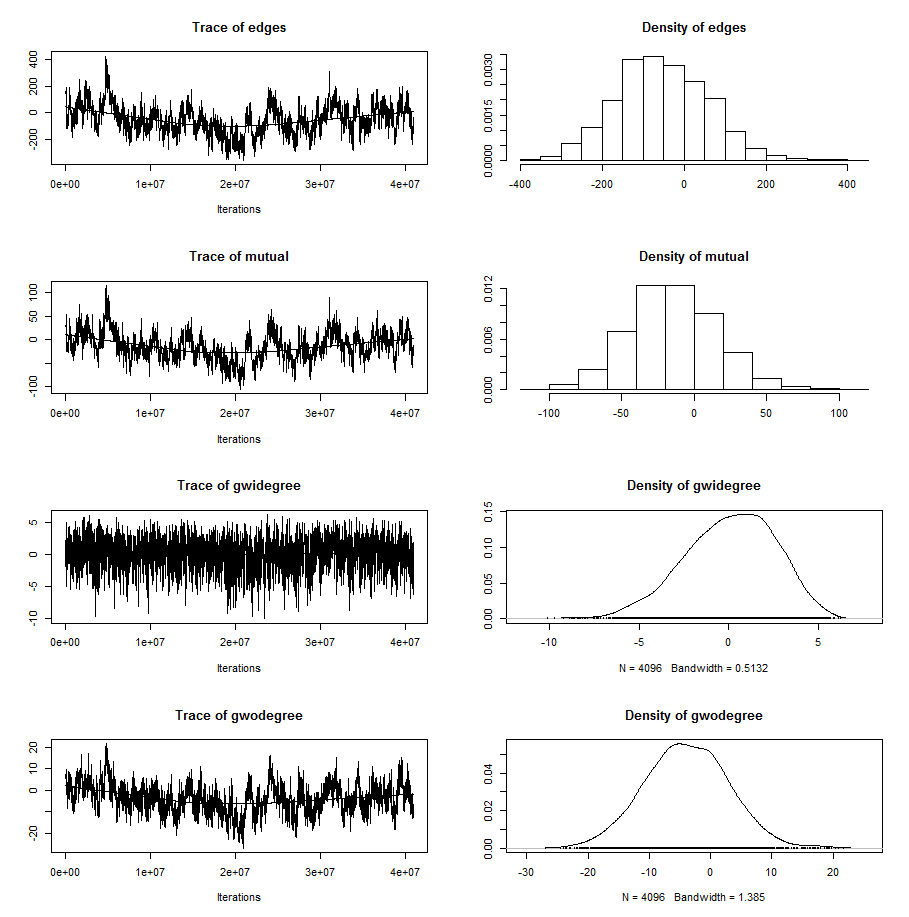
\includegraphics[width=1\textwidth]{../ERGM/mcmcdiagergm3.png}
	\caption{MCMC Diagnose von Modell 1}
	\label{fig:mcmc.diag.model1}
\end{figure}


Bei den Goodness of Fit Plots in Abbildung \ref{fig:gof.model1} fällt auf: out degree und minimum geodesic distance sind sehr gut getroffen, aber die esp- Statistiken werden bei kleinen Werten stark überschätzt und danach unterschätzt. Der In-Degree wird vor allem bei den Werten 1 und 2 nicht getroffen. 
Mögliche Lösung: Variation des decay-Parameters? Leider tendeiert das Modell für größere decay Werte zur Degeneration wie auch in \citet{goodreau2008statnet} berichtet.

\begin{figure}[ht]
	\centering
		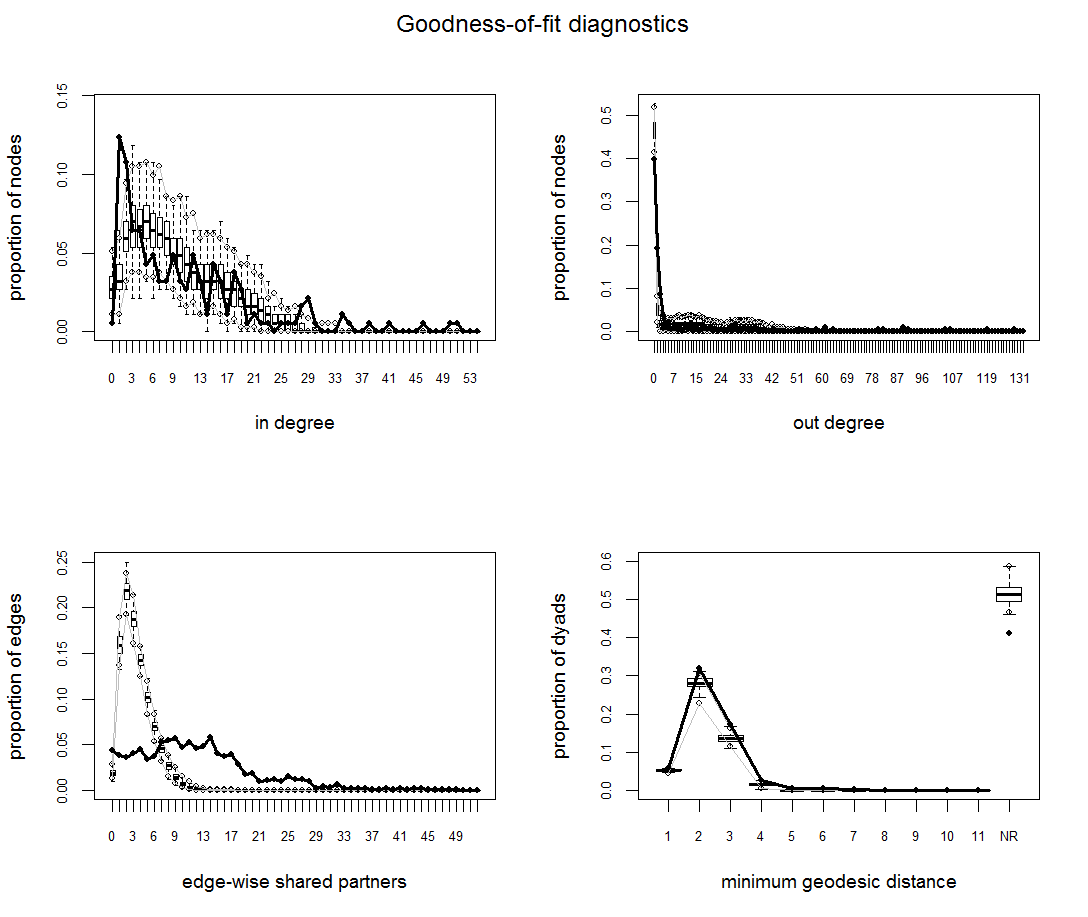
\includegraphics[width=1\textwidth]{../ERGM/GOF3.png}
	\caption{Goodness of Fit von Modell 1}
	\label{fig:gof.model1}
\end{figure}


\section{Interpretation der Parameter}

Für den nachfolgenden wird der Begriff der \emph{Change Statistiken} benötigt: $\theta^T\delta_g(x)_{ij}$ ist der Vektor der sogenannten \emph{Change-Statistiken}
 
$$ \theta^T\delta_g(x)_{ij} = g(x^+_{ij}) - g(x^-_{ij}) $$

wobei $x^+_{ij}$ und $x^-_{ij}$ die jeweiligen Netzwerke sind, die man erhält, wenn man in einem bestimmten Netzwerk $x$ die Kannte $x_{ij}$ als gegeben ($x_{ij} = 1$) oder abwesend ($x_{ij}= 0$) festlegt. $\theta^T\delta_g(x)_{ij}$ misst also den Wert der Veränderung der Statistiken $g(x)$ zwischen dem ansonsten gleichen Netzwerken mit und ohne der Kante $x_{ij}$.


Für eine einfache Interpretation der Modellparameter lässt sich Modellgleichung \ref{eq:ergm} nun umschreiben zu 
\begin{equation}
	logit\left[P_{\theta, \mathcal{X}}(X_{ij} = 1 | X^c_{ij} = x^c_{ij})\right] = \theta^T\delta_g(x)_{ij}.
	\label{eq:change}
\end{equation}
Die logit Funktion ist definiert als $logit(p) = log\left[p/(1-p)\right]$ und $X^c_{ij}$ repräsentiert das restliche Netzwerk ohne die einzelnen Variable $X_{ij}$. 

Die Wahrscheinlichkeit auf der linken Seite von Gleichung \ref{eq:change} hängt nun nur noch von den Change Statistiken $\theta^T\delta_g(x)_{ij}$ ab und nicht mehr von den Netzwerkstatistiken $g(x^+_{ij})$ und $g(x^-_{ij})$ selbst.
Hierdurch ergibt sich eine einfache Interpretation der Modellparameter $\theta$. Jedes Element aus $\theta$ lässt sich nun interpretieren als der Anstieg der bedingten log-odds des Netzwerkes, pro Anstieg des entsprechenden Elements aus $g(x)$, der aus dem Wechsel von $X_{ij}$ von $0$ zu $1$ resultiert \citep{hunter2008ergm}.

\newpage







\bibliographystyle{dcu}
\bibliography{literatur}
\newpage
\listoffigures
\newpage
\listoftables




\chapter*{Anhang}
{
\footnotesize
\begin{longtable}{rllrrr}

  \hline
 row & Reporter\_Name & Partner\_Name & Year & Value & PRIO\_Weapons\_Code \\ 
  \hline
  328 & Albania & Albania & 2005 & 3366.00 & 223 \\ 
  346 & Albania & Albania & 2006 & 13355.00 & 223 \\ 
  4143 & Australia & Australia & 2004 & 586143.00 & 210 \\ 
  4161 & Australia & Australia & 2004 & 13241.00 & 223 \\ 
  4183 & Australia & Australia & 2004 & 721.00 & 227 \\ 
  4211 & Australia & Australia & 2004 & 4693884.00 & 260 \\ 
  4224 & Australia & Australia & 2004 & 48697.00 & 417 \\ 
  4257 & Australia & Australia & 2005 & 15054.00 & 210 \\ 
  4318 & Australia & Australia & 2005 & 3180066.00 & 260 \\ 
  4329 & Australia & Australia & 2005 & 639.00 & 417 \\ 
  4362 & Australia & Australia & 2006 & 42325.00 & 210 \\ 
  4396 & Australia & Australia & 2006 & 31458.00 & 227 \\ 
  4422 & Australia & Australia & 2006 & 2473903.00 & 260 \\ 
  4435 & Australia & Australia & 2006 & 682288.00 & 417 \\ 
  4466 & Australia & Australia & 2007 & 1431868.00 & 210 \\ 
  4528 & Australia & Australia & 2007 & 4132772.00 & 260 \\ 
  4579 & Australia & Australia & 2008 & 869812.00 & 210 \\ 
  4641 & Australia & Australia & 2008 & 2870285.00 & 260 \\ 
  4653 & Australia & Australia & 2008 & 6652.00 & 417 \\ 
  4692 & Australia & Australia & 2009 & 37710.00 & 210 \\ 
  4731 & Australia & Australia & 2009 & 8857.00 & 227 \\ 
  4758 & Australia & Australia & 2009 & 857590.00 & 260 \\ 
  4804 & Australia & Australia & 2010 & 19084.00 & 210 \\ 
  4839 & Australia & Australia & 2010 & 13162.00 & 227 \\ 
  4866 & Australia & Australia & 2010 & 580277.00 & 260 \\ 
  4876 & Australia & Australia & 2010 & 1836.00 & 417 \\ 
  4915 & Australia & Australia & 2011 & 283630.00 & 210 \\ 
  4955 & Australia & Australia & 2011 & 33770.00 & 227 \\ 
  4985 & Australia & Australia & 2011 & 4529308.00 & 260 \\ 
  9934 & Belgium & Belgium & 2010 & 1056327.00 & 223 \\ 
  9951 & Belgium & Belgium & 2010 & 27087.00 & 227 \\ 
  11189 & Bosnia-Herzegovina & Bosnia-Herzegovina & 2003 & 94087.00 & 417 \\ 
  13542 & Bulgaria & Bulgaria & 2011 & 472000.00 & 200 \\ 
  15412 & Canada & Canada & 2002 & 2397.00 & 227 \\ 
  15434 & Canada & Canada & 2002 & 823.00 & 260 \\ 
  15455 & Canada & Canada & 2002 & 91030.00 & 417 \\ 
  15567 & Canada & Canada & 2003 & 13484.00 & 260 \\ 
  15586 & Canada & Canada & 2003 & 194230.00 & 417 \\ 
  15626 & Canada & Canada & 2004 & 11122.00 & 210 \\ 
  15698 & Canada & Canada & 2004 & 7179.00 & 260 \\ 
  15721 & Canada & Canada & 2004 & 221463.00 & 417 \\ 
  15848 & Canada & Canada & 2005 & 32756.00 & 417 \\ 
  15937 & Canada & Canada & 2006 & 7181.00 & 227 \\ 
  15967 & Canada & Canada & 2006 & 1616.00 & 260 \\ 
  15997 & Canada & Canada & 2006 & 355640.00 & 417 \\ 
  16085 & Canada & Canada & 2007 & 13454.00 & 227 \\ 
  16146 & Canada & Canada & 2007 & 208218.00 & 417 \\ 
  16178 & Canada & Canada & 2007 & 12.00 & 418 \\ 
  16201 & Canada & Canada & 2008 & 1000.00 & 210 \\ 
  16242 & Canada & Canada & 2008 & 60664.00 & 227 \\ 
  16268 & Canada & Canada & 2008 & 250.00 & 260 \\ 
  16292 & Canada & Canada & 2008 & 35525.00 & 417 \\ 
  16383 & Canada & Canada & 2009 & 23435.00 & 227 \\ 
  16408 & Canada & Canada & 2009 & 45762.00 & 260 \\ 
  16428 & Canada & Canada & 2009 & 24582.00 & 417 \\ 
  16509 & Canada & Canada & 2010 & 34898.00 & 223 \\ 
  16532 & Canada & Canada & 2010 & 78136.00 & 227 \\ 
  16566 & Canada & Canada & 2010 & 9716.00 & 260 \\ 
  16593 & Canada & Canada & 2010 & 938822.00 & 417 \\ 
  16691 & Canada & Canada & 2011 & 19734.00 & 227 \\ 
  16722 & Canada & Canada & 2011 & 6694.00 & 260 \\ 
  16745 & Canada & Canada & 2011 & 11456.00 & 417 \\ 
  16780 & Canada & Canada & 2011 & 10.00 & 418 \\ 
  21855 & Cyprus & Cyprus & 2001 & 157920.00 & 418 \\ 
  21957 & Cyprus & Cyprus & 2003 & 606.00 & 418 \\ 
  24043 & Czech Republic & Czech Republic & 2004 & 133060.00 & 200 \\ 
  28760 & Estonia & Estonia & 2007 & 5085.00 & 417 \\ 
  32299 & France & France & 2000 & 43412.00 & 223 \\ 
  32350 & France & France & 2000 & 361290.00 & 417 \\ 
  32375 & France & France & 2000 & 619970.00 & 418 \\ 
  32398 & France & France & 2001 & 89525.00 & 223 \\ 
  32424 & France & France & 2001 & 6714.00 & 227 \\ 
  32453 & France & France & 2001 & 82811.00 & 417 \\ 
  32473 & France & France & 2001 & 125337.00 & 418 \\ 
  32501 & France & France & 2002 & 16244.00 & 223 \\ 
  32525 & France & France & 2002 & 11601.00 & 227 \\ 
  32557 & France & France & 2002 & 11601.00 & 417 \\ 
  32577 & France & France & 2002 & 475712.00 & 418 \\ 
  32606 & France & France & 2003 & 2723.00 & 223 \\ 
  32632 & France & France & 2003 & 2723.00 & 227 \\ 
  32662 & France & France & 2003 & 1078653.00 & 417 \\ 
  32683 & France & France & 2003 & 1070481.00 & 418 \\ 
  32703 & France & France & 2004 & 990720.00 & 223 \\ 
  32728 & France & France & 2004 & 1937735.00 & 227 \\ 
  32759 & France & France & 2004 & 748867.00 & 417 \\ 
  32784 & France & France & 2004 & 1264627.00 & 418 \\ 
  32898 & France & France & 2006 & 79966.00 & 223 \\ 
  32925 & France & France & 2006 & 82722.00 & 227 \\ 
  32957 & France & France & 2006 & 24817.00 & 417 \\ 
  33016 & France & France & 2007 & 55657.00 & 223 \\ 
  33039 & France & France & 2007 & 131821.00 & 227 \\ 
  33080 & France & France & 2007 & 90809.00 & 417 \\ 
  33106 & France & France & 2007 & 29292.00 & 418 \\ 
  33130 & France & France & 2008 & 15382.00 & 223 \\ 
  33154 & France & France & 2008 & 153832.00 & 227 \\ 
  33183 & France & France & 2008 & 21535.00 & 417 \\ 
  33208 & France & France & 2008 & 24613.00 & 418 \\ 
  33237 & France & France & 2009 & 8619.00 & 223 \\ 
  33261 & France & France & 2009 & 20111.00 & 227 \\ 
  33293 & France & France & 2009 & 31603.00 & 417 \\ 
  33320 & France & France & 2009 & 301662.00 & 418 \\ 
  33406 & France & France & 2010 & 8121.00 & 417 \\ 
  33425 & France & France & 2010 & 2706.00 & 418 \\ 
  33472 & France & France & 2011 & 2782.00 & 227 \\ 
  33501 & France & France & 2011 & 11132.00 & 417 \\ 
  60737 & Malaysia & Malaysia & 2010 & 67114.00 & 418 \\ 
  68357 & New Zealand & New Zealand & 2008 & 5021.00 & 223 \\ 
  68378 & New Zealand & New Zealand & 2008 & 4422.00 & 227 \\ 
  68708 & New Zealand & New Zealand & 2011 & 648.00 & 227 \\ 
  84157 & Slovakia & Slovakia & 2002 & 115.00 & 260 \\ 
  84174 & Slovakia & Slovakia & 2002 & 28790.00 & 417 \\ 
  84230 & Slovakia & Slovakia & 2003 & 11114.00 & 260 \\ 
  84249 & Slovakia & Slovakia & 2003 & 37417.00 & 417 \\ 
  95974 & Thailand & Thailand & 2007 & 15078.00 & 210 \\ 
  96004 & Thailand & Thailand & 2007 & 320.00 & 227 \\ 
  96375 & Thailand & Thailand & 2011 & 11096.00 & 227 \\ 
  101434 & United Kingdom & United Kingdom & 2000 & 2663869.00 & 223 \\ 
  101462 & United Kingdom & United Kingdom & 2000 & 1450872.00 & 227 \\ 
  101507 & United Kingdom & United Kingdom & 2000 & 216810.00 & 418 \\ 
  101542 & United Kingdom & United Kingdom & 2001 & 3715829.00 & 223 \\ 
  101569 & United Kingdom & United Kingdom & 2001 & 503356.00 & 227 \\ 
  101646 & United Kingdom & United Kingdom & 2002 & 1602392.00 & 223 \\ 
  101671 & United Kingdom & United Kingdom & 2002 & 1051572.00 & 227 \\ 
  101702 & United Kingdom & United Kingdom & 2002 & 177831.00 & 417 \\ 
  101718 & United Kingdom & United Kingdom & 2002 & 374054.00 & 418 \\ 
  101752 & United Kingdom & United Kingdom & 2003 & 6230061.00 & 223 \\ 
  101782 & United Kingdom & United Kingdom & 2003 & 1625580.00 & 227 \\ 
  101811 & United Kingdom & United Kingdom & 2003 & 15105.00 & 417 \\ 
  101859 & United Kingdom & United Kingdom & 2004 & 8316031.00 & 223 \\ 
  101883 & United Kingdom & United Kingdom & 2004 & 2539407.00 & 227 \\ 
  101932 & United Kingdom & United Kingdom & 2004 & 6603.00 & 418 \\ 
  101967 & United Kingdom & United Kingdom & 2005 & 7487298.00 & 223 \\ 
  101996 & United Kingdom & United Kingdom & 2005 & 2504286.00 & 227 \\ 
  102027 & United Kingdom & United Kingdom & 2005 & 53655.00 & 417 \\ 
  102045 & United Kingdom & United Kingdom & 2005 & 6252.00 & 418 \\ 
  102085 & United Kingdom & United Kingdom & 2006 & 7520540.00 & 223 \\ 
  102115 & United Kingdom & United Kingdom & 2006 & 3570588.00 & 227 \\ 
  102148 & United Kingdom & United Kingdom & 2006 & 49884.00 & 417 \\ 
  102193 & United Kingdom & United Kingdom & 2007 & 7235351.00 & 223 \\ 
  102222 & United Kingdom & United Kingdom & 2007 & 3207893.00 & 227 \\ 
  102255 & United Kingdom & United Kingdom & 2007 & 22582.00 & 417 \\ 
  102305 & United Kingdom & United Kingdom & 2008 & 3432365.00 & 223 \\ 
  102333 & United Kingdom & United Kingdom & 2008 & 983561.00 & 227 \\ 
  102417 & United Kingdom & United Kingdom & 2009 & 3660097.00 & 223 \\ 
  102442 & United Kingdom & United Kingdom & 2009 & 1124347.00 & 227 \\ 
  102483 & United Kingdom & United Kingdom & 2009 & 22303.00 & 417 \\ 
  102540 & United Kingdom & United Kingdom & 2010 & 4121609.00 & 223 \\ 
  102564 & United Kingdom & United Kingdom & 2010 & 732804.00 & 227 \\ 
  102647 & United Kingdom & United Kingdom & 2011 & 4910676.00 & 223 \\ 
  102670 & United Kingdom & United Kingdom & 2011 & 1131532.00 & 227 \\ 
  102699 & United Kingdom & United Kingdom & 2011 & 25154.00 & 417 \\ 
   \hline
	\caption{Auflistung der gelöschten Schleifen im Datensatz}
\end{longtable}

 }


\chapter*{Eidesstattliche Erklärung}

Ich erklären hiermit, dass ich diese Arbeit ohne fremde Hilfe angefertigt und nur die im Literaturverzeichnis aufgeführten Quellen und Hilfsmittel benutzt habe. Diese Arbeit wurde noch nicht zu anderen prüfungsrelevanten Zwecken vorgelegt.\\[1.5cm]

\noindent ..............................................
\qquad\qquad\qquad\qquad\qquad
....................................................\\[0.5mm]
\textit{Ort, Datum}
\qquad\qquad\qquad\qquad\qquad\qquad\qquad\qquad\qquad
\textit{Felix Loewe}














\end{document}


